\section{EXPERIMENTS}
\label{sec:experiments}

\subsection{Setup}
\label{sec:setup}
\readorder{9}

\paragraph{Sections.}
We fit DISCELL to four sections profiled with the same imaging-based assay and gene panel of about five thousand genes \citep{janesick2023}: an ovarian cancer section preserved by formalin fixation and paraffin embedding (FFPE), our primary section \citep{tenx_ovarian_ffpe}; a lung cancer section, also FFPE \citep{tenx_lung_ffpe}; a fresh-frozen ovarian cancer section, with about eight times the median count per cell \citep{tenx_ovary_ff}; and a core of a paediatric lung tissue microarray (TMA) from GEO series GSE315411 \citep{williamskatek2026fishing}. A serial section of the same TMA core on a second slide is the held-out section: no model is fitted to it, and it is read only through the model fitted on its neighbour. The sections range from about seventy thousand to over a million cells (\cref{tab:sections}).

\paragraph{Labels.}
\flag{MERGE}{repeats 2.1 on lineage labels and Unassigned; keep the curated vs clustered split} Every section carries lineage-level labels, in which states and locations are merged into their lineage (\cref{sec:setting}). On the ovarian FFPE section and the TMA they are derived from curated annotations, and on the other two from marker-annotated clusters; the mappings were fixed before any fit at lineage labels. Cells without a usable lineage label form one class, which enters training like any other and is never a target of evaluation.

\paragraph{Graph, kernel and image.}
\flag{CUT}{repeats 2.1; one clause in Configuration suffices} The graph is Delaunay adjacency pruned at $40\um$, the leakage kernel is $\beta$ with $\tau = 20\um$, and the image descriptor is the KRONOS embedding of the four-channel $128\um$ field with the $25\um$ disc over the cell set to zero, on every section (\cref{sec:setting}, \cref{app:graph,app:image}).

\paragraph{Configuration.}
\flag{REVIEWER}{keep: kappa 0.1 is a working point, not selected by reconstruction (decided 09-29)} One configuration is used on every section (\cref{tab:architecture}): a KL warm-up of the response over its first thirty epochs, the adversary with its composition term weighted three times its image term, in the heads' loss and in the encoder's, $\kappa = 0.1$ as the operating point, and a budget of $500$ epochs with patience $40$. Only $\alphaz$ changes between sections, apart from smaller tiles on the TMA core (below), because it is set to $\tfrac12 \cdot 1/\lbar$ with $\lbar$ the section's count scale: its median total count, with the primary section's value fixed during development. The operating point $\kappa = 0.1$ is where the analyses that need a single fit are read, not an estimate of the leak fraction. It was taken before the full sweep, to match the typical misassignment on this platform, about a tenth of a cell's transcripts \citep{yang2025mistic}, and kept after it, because on the primary section it lies at the end of the plateau of held-out reconstruction, where the loadings agree best across seeds and the mirror diagnostic (\cref{sec:selection}) is already below its level at $\kappa = 0$. Held-out reconstruction scores the fit as an autoencoder and favours small $\kappa$, so it describes the point rather than selecting it, and no claim rests on the choice: every claimed contrast is reported across the sweep with its breakdown point (\cref{sec:sweep}).

\paragraph{Splits, seeds and read-outs.}
Each section is cut into contiguous tiles of at most $4{,}096$ cells ($2{,}048$ on the TMA core), and $15\%$ of the tiles are held out (\cref{app:tiles}). Every final configuration is fitted from three random seeds, each of which also redraws the held-out split, and every fit is read at its accepted checkpoint. A readout is reported as the mean over seeds with its range, and, where a sampling interval is needed, with a spatial block bootstrap over tiles (\cref{sec:sweep}). The leakage sweep refits the same configuration at every $\kappa \in \{0, 0.05, 0.1, 0.2, 0.3, 0.4\}$ with three seeds each. Every readout is defined in \cref{app:readouts}.

\paragraph{Baselines.}
We compare with resolVI \citep{ergen2025}, SIMVI \citep{dong2025simvi}, MintFlow \citep{akbarnejad2025mintflow} and Cellina \citep{moeed2026cellina}, each at its published defaults, on our graph wherever the method accepts an external one, and on whole sections only (\cref{tab:baselines}). They were not tuned, while DISCELL's weights were calibrated on the sections reported here, two or three seeds per setting: $\alphaz$ over four values on the primary section, $\alphaw$ over five multiples of $1/\lbar$ against $0.1$ on the primary section and the TMA core, and over two on the fresh-frozen section, and the adversary's head steps, head width, ensemble size and composition weight on the primary section, the weight confirmed on the TMA core and the fresh-frozen section (\cref{app:sensitivity}). Each comparison method is fitted as its software is designed, on every cell of the section with at least five counts, held-out tiles included; all methods are then scored by the same read-outs on their intrinsic latent, on our held-out cells and labels. Cellina removes a spatial-domain label from its intrinsic latent adversarially; our sections have none, so it is run without that adversary and, in a second row, with our niche label in the domain's place. SIMVI, MintFlow and Cellina split each cell into an intrinsic latent and a context latent, as DISCELL does; resolVI models the contamination of a cell's counts by its neighbours as a mixture and keeps a single cell latent, so it is a reference for the intrinsic side, not an intrinsic/context split. MintFlow is fitted on the TMA core and on the whole lung FFPE and ovarian FFPE sections, and SIMVI on the TMA core and its serial section. Their other whole-section fits could not be run on the resources currently available, for measured reasons (\cref{tab:baselines}): SIMVI ran out of memory on a 24 GB GPU within minutes on the lung FFPE, ovarian FFPE and fresh-frozen sections, and MintFlow, on the fresh-frozen section's $1.16$ million cells, was killed for lack of host memory while setting up its data, before training, on a 125 GB host.

\subsection{Recovery on Simulated Sections}
\label{sec:synthetic}
\readorder{8}

\flag{TRIM}{number-dense; keep headline recovery and misspecification, ranges to app:synthetic} On sections simulated from the model's own generative story, with types that cluster in space, a response linear in the neighbour composition and a planted leak fraction of $0$ or $0.2$, the final configuration recovers what was planted (\cref{app:synthetic}, \cref{tab:synthetic}). Over nine fits per planted fraction, the intrinsic state agrees with the planted type about as well as clusters of the counts do or better (NMI $0.80$ to $0.96$, against $0.69$ to $0.93$; below them on one fit of the eighteen, $0.80$ against $0.83$), the response correlates with the planted one (first canonical correlation $0.83$ to $0.95$), the fitted loadings recover the planted ones (largest principal-angle cosine $0.63$ to $0.99$, above the $95$th percentile of random subspaces, $0.37$ to $0.38$, in every fit), and the intrinsic state carries almost none of the planted niche (within-type $R^2$ of composition at most $0.04$, against $0.11$ to $0.19$ without the adversary). Fitted at a wrong leak fraction, anywhere from $0$ to $0.4$ on sections planted at $0.2$, the same reads move little. A second simulation plants a per-cell response that the niche does not predict; the response channel does not detect it at the operating point (\cref{sec:results-w}).

\subsection{Model Quality Across Four Tissues}
\label{sec:results-quality}
\readorder{8}
% manifest row 1: envelope table (recon, NMI, mirror, cycle_z/cycle_w, I(niche;w), transport, atlas)

\flag{TRIM}{transport and programme numbers repeat 3.5; keep type, cycle, niche, mirror, serial} \Cref{tab:headline} gives the model on every section. The intrinsic state keeps the cell type, with a normalised mutual information of $0.62$ to $0.74$ with the lineage labels, and it carries the cell cycle while the response does not: on the most strongly cycling tenth of cells, $\vz$ explains $19$ to $76\%$ of the variance of the cycle scores and $\vw$ at most $1\%$ in any seed, below $0.01$ everywhere; the seed envelope of its intervals contains zero on every fitted section (\cref{tab:headline-full}), although single seeds on the ovarian, lung and fresh-frozen sections exclude zero at these small values. The response carries the niche, with $0.47$ to $0.60$ nats of information about it beyond a within-type permutation floor, and the context does not mirror the intrinsic state (mirror $R^2$ of $0.03$ to $0.09$; \cref{sec:selection}). The first response programme is reproduced across seeds with a cosine of $0.82$ to $0.97$, and the response's transported prediction of how a type's expression differs between two niches recovers $0.65$ to $0.73$ of the part of that difference that is reproducible between halves of the cells (\cref{sec:results-w}). The model fitted to the TMA core reads its serial section, which it never saw, as it reads the core: the agreement with type is $0.61$ against $0.62$ and the cycle $R^2$ of $\vz$ $0.50$ on both.

\flag{KEEP-CORE}{tab:headline, the one results table in the main text} % Generated table: tab:headline. DO NOT EDIT BY HAND; regenerate instead.
% Command: python scripts/paper_tables.py
% Generated: 2026-09-29 16:44:01 (results frozen 2026-09-29 15:07:21, last line of scripts/logs/unassigned_2026-09-28/queue.log)
%
% Sources read (modification time):
%   data/datasets/gse315411_pdltma06_11_prime_solo/experiments/envelope_table_ci_at_best.md  (2026-09-29 09:46:56)
%   data/datasets/gse315411_pdltma06_11_prime_solo/runs/finalL_s0/crossslide/gse315411_pdltma06_10_prime_dual.json  (2026-09-28 16:13:47)
%   data/datasets/gse315411_pdltma06_11_prime_solo/runs/finalL_s1/crossslide/gse315411_pdltma06_10_prime_dual.json  (2026-09-28 16:24:14)
%   data/datasets/gse315411_pdltma06_11_prime_solo/runs/finalL_s2/crossslide/gse315411_pdltma06_10_prime_dual.json  (2026-09-28 16:34:44)
%   data/datasets/xenium_prime_human_lung_cancer_ffpe/experiments/envelope_table_ci_at_best.md  (2026-09-29 09:46:56)
%   data/datasets/xenium_prime_human_ovary_ff/experiments/envelope_table_ci_at_best.md  (2026-09-29 09:46:56)
%   data/datasets/xenium_prime_ovarian_cancer_ffpe/experiments/envelope_table_ci_at_best.md  (2026-09-29 09:46:56)
%
% Reading convention:
%   accepted checkpoint; 3-seed mean with [min, max] over finalL_s0-s2; tile-bootstrap 95 % CI
%   where the source has one (envelope of the per-seed intervals); Unassigned excluded as a
%   target of every read; cycle reads on the label-free top-decile cycling set (q90); rounding
%   half-up from the value in the file; the serial section's values come from the core's three
%   fits read on it
%
% Provenance (row / column -> file : key):
%   Reconstruction / Ovarian FFPE: data/datasets/xenium_prime_ovarian_cancer_ffpe/experiments/envelope_table_ci_at_best.md : row 'held-out reconstruction (nats/count)' (mean; min, max; CI column)
%   Reconstruction / Lung FFPE: data/datasets/xenium_prime_human_lung_cancer_ffpe/experiments/envelope_table_ci_at_best.md : row 'held-out reconstruction (nats/count)' (mean; min, max; CI column)
%   Reconstruction / Ovarian FF: data/datasets/xenium_prime_human_ovary_ff/experiments/envelope_table_ci_at_best.md : row 'held-out reconstruction (nats/count)' (mean; min, max; CI column)
%   Reconstruction / TMA core: data/datasets/gse315411_pdltma06_11_prime_solo/experiments/envelope_table_ci_at_best.md : row 'held-out reconstruction (nats/count)' (mean; min, max; CI column)
%   Reconstruction / TMA serial: held_out_section.recon_val_targets over seeds 0-2 (runs/finalL_s{0,1,2}/crossslide/gse315411_pdltma06_10_prime_dual.json); mean checked against data/datasets/gse315411_pdltma06_11_prime_solo/experiments/envelope_table_ci_at_best.md : 'held-out reconstruction (nats/count)' held-out mean
%   NMI of $\vz$ with the type / Ovarian FFPE: data/datasets/xenium_prime_ovarian_cancer_ffpe/experiments/envelope_table_ci_at_best.md : row 'NMI vs the type labels' (mean; min, max; CI column)
%   NMI of $\vz$ with the type / Lung FFPE: data/datasets/xenium_prime_human_lung_cancer_ffpe/experiments/envelope_table_ci_at_best.md : row 'NMI vs the type labels' (mean; min, max; CI column)
%   NMI of $\vz$ with the type / Ovarian FF: data/datasets/xenium_prime_human_ovary_ff/experiments/envelope_table_ci_at_best.md : row 'NMI vs the type labels' (mean; min, max; CI column)
%   NMI of $\vz$ with the type / TMA core: data/datasets/gse315411_pdltma06_11_prime_solo/experiments/envelope_table_ci_at_best.md : row 'NMI vs the type labels' (mean; min, max; CI column)
%   NMI of $\vz$ with the type / TMA serial: held_out_section.nmi_targets over seeds 0-2 (runs/finalL_s{0,1,2}/crossslide/gse315411_pdltma06_10_prime_dual.json); mean checked against data/datasets/gse315411_pdltma06_11_prime_solo/experiments/envelope_table_ci_at_best.md : 'NMI vs the type labels' held-out mean
%   Mirror $R^2$ / Ovarian FFPE: data/datasets/xenium_prime_ovarian_cancer_ffpe/experiments/envelope_table_ci_at_best.md : row 'mirror R²' (mean; min, max; CI column)
%   Mirror $R^2$ / Lung FFPE: data/datasets/xenium_prime_human_lung_cancer_ffpe/experiments/envelope_table_ci_at_best.md : row 'mirror R²' (mean; min, max; CI column)
%   Mirror $R^2$ / Ovarian FF: data/datasets/xenium_prime_human_ovary_ff/experiments/envelope_table_ci_at_best.md : row 'mirror R²' (mean; min, max; CI column)
%   Mirror $R^2$ / TMA core: data/datasets/gse315411_pdltma06_11_prime_solo/experiments/envelope_table_ci_at_best.md : row 'mirror R²' (mean; min, max; CI column)
%   Mirror $R^2$ / TMA serial: held_out_section.mirror.r2 over seeds 0-2 (runs/finalL_s{0,1,2}/crossslide/gse315411_pdltma06_10_prime_dual.json); mean checked against data/datasets/gse315411_pdltma06_11_prime_solo/experiments/envelope_table_ci_at_best.md : 'mirror R²' held-out mean
%   Cycle $R^2$ of $\vz$ / Ovarian FFPE: data/datasets/xenium_prime_ovarian_cancer_ffpe/experiments/envelope_table_ci_at_best.md : row 'cycle R² (z, top-decile set)' (mean; min, max; CI column)
%   Cycle $R^2$ of $\vz$ / Lung FFPE: data/datasets/xenium_prime_human_lung_cancer_ffpe/experiments/envelope_table_ci_at_best.md : row 'cycle R² (z, top-decile set)' (mean; min, max; CI column)
%   Cycle $R^2$ of $\vz$ / Ovarian FF: data/datasets/xenium_prime_human_ovary_ff/experiments/envelope_table_ci_at_best.md : row 'cycle R² (z, top-decile set)' (mean; min, max; CI column)
%   Cycle $R^2$ of $\vz$ / TMA core: data/datasets/gse315411_pdltma06_11_prime_solo/experiments/envelope_table_ci_at_best.md : row 'cycle R² (z, top-decile set)' (mean; min, max; CI column)
%   Cycle $R^2$ of $\vz$ / TMA serial: held_out_section.cycle_r2_z_q90 over seeds 0-2 (runs/finalL_s{0,1,2}/crossslide/gse315411_pdltma06_10_prime_dual.json); mean checked against data/datasets/gse315411_pdltma06_11_prime_solo/experiments/envelope_table_ci_at_best.md : 'cycle R² (z, top-decile set)' held-out mean
%   Cycle $R^2$ of $\vw$ / Ovarian FFPE: data/datasets/xenium_prime_ovarian_cancer_ffpe/experiments/envelope_table_ci_at_best.md : row 'cycle R² (w, top-decile set)' (mean; min, max; CI column)
%   Cycle $R^2$ of $\vw$ / Lung FFPE: data/datasets/xenium_prime_human_lung_cancer_ffpe/experiments/envelope_table_ci_at_best.md : row 'cycle R² (w, top-decile set)' (mean; min, max; CI column)
%   Cycle $R^2$ of $\vw$ / Ovarian FF: data/datasets/xenium_prime_human_ovary_ff/experiments/envelope_table_ci_at_best.md : row 'cycle R² (w, top-decile set)' (mean; min, max; CI column)
%   Cycle $R^2$ of $\vw$ / TMA core: data/datasets/gse315411_pdltma06_11_prime_solo/experiments/envelope_table_ci_at_best.md : row 'cycle R² (w, top-decile set)' (mean; min, max; CI column)
%   Cycle $R^2$ of $\vw$ / TMA serial: held_out_section.cycle_r2_w_q90 over seeds 0-2 (runs/finalL_s{0,1,2}/crossslide/gse315411_pdltma06_10_prime_dual.json); mean checked against data/datasets/gse315411_pdltma06_11_prime_solo/experiments/envelope_table_ci_at_best.md : 'cycle R² (w, top-decile set)' held-out mean
%   $\I(\text{niche}; \vw)$ excess / Ovarian FFPE: data/datasets/xenium_prime_ovarian_cancer_ffpe/experiments/envelope_table_ci_at_best.md : row 'I(niche; w) excess over within-type floor (nats)' (mean; min, max; CI column)
%   $\I(\text{niche}; \vw)$ excess / Lung FFPE: data/datasets/xenium_prime_human_lung_cancer_ffpe/experiments/envelope_table_ci_at_best.md : row 'I(niche; w) excess over within-type floor (nats)' (mean; min, max; CI column)
%   $\I(\text{niche}; \vw)$ excess / Ovarian FF: data/datasets/xenium_prime_human_ovary_ff/experiments/envelope_table_ci_at_best.md : row 'I(niche; w) excess over within-type floor (nats)' (mean; min, max; CI column)
%   $\I(\text{niche}; \vw)$ excess / TMA core: data/datasets/gse315411_pdltma06_11_prime_solo/experiments/envelope_table_ci_at_best.md : row 'I(niche; w) excess over within-type floor (nats)' (mean; min, max; CI column)
%   $\I(\text{niche}; \vw)$ excess / TMA serial: not evaluated on the held-out section (envelope held-out n = 0)
%   Transport / Ovarian FFPE: withheld (would be data/datasets/xenium_prime_ovarian_cancer_ffpe/experiments/envelope_table_ci_at_best.md : row 'transport, mean read: fraction of ceiling (trusted)')
%   Transport / Lung FFPE: withheld (would be data/datasets/xenium_prime_human_lung_cancer_ffpe/experiments/envelope_table_ci_at_best.md : row 'transport, mean read: fraction of ceiling (trusted)')
%   Transport / Ovarian FF: withheld (would be data/datasets/xenium_prime_human_ovary_ff/experiments/envelope_table_ci_at_best.md : row 'transport, mean read: fraction of ceiling (trusted)')
%   Transport / TMA core: withheld (would be data/datasets/gse315411_pdltma06_11_prime_solo/experiments/envelope_table_ci_at_best.md : row 'transport, mean read: fraction of ceiling (trusted)')
%   Transport / TMA serial: not evaluated on the held-out section (envelope held-out n = 0)
%   Atlas cross-seed cosine / Ovarian FFPE: data/datasets/xenium_prime_ovarian_cancer_ffpe/experiments/envelope_table_ci_at_best.md : row 'atlas cross-seed axis-1 cosine' (mean; min, max; CI column)
%   Atlas cross-seed cosine / Lung FFPE: data/datasets/xenium_prime_human_lung_cancer_ffpe/experiments/envelope_table_ci_at_best.md : row 'atlas cross-seed axis-1 cosine' (mean; min, max; CI column)
%   Atlas cross-seed cosine / Ovarian FF: data/datasets/xenium_prime_human_ovary_ff/experiments/envelope_table_ci_at_best.md : row 'atlas cross-seed axis-1 cosine' (mean; min, max; CI column)
%   Atlas cross-seed cosine / TMA core: data/datasets/gse315411_pdltma06_11_prime_solo/experiments/envelope_table_ci_at_best.md : row 'atlas cross-seed axis-1 cosine' (mean; min, max; CI column)
%   Atlas cross-seed cosine / TMA serial: not evaluated on the held-out section (envelope held-out n = 0)
%
% Checks and notes:
%   - Ovarian FFPE: the envelope skipped null atlas cross-seed cosines for `finalL_s1`,
%     `finalL_s2`; the cell is over the seed pairs that exist.
%   - Ovarian FF: the envelope skipped null atlas cross-seed cosines for `finalL_s0`,
%     `finalL_s2`; the cell is over the seed pairs that exist.
%   - The held-out section (TMA serial) is read through the models fitted on the core; the
%     envelope gives it a mean only, so the range is recomputed from the three per-seed
%     cross-slide files and the mean is checked against the envelope. It has no tile-bootstrap
%     interval, and I(niche; w), transport and atlas are not read on it ('--', not pending: no
%     queue computes them).
%   - Values are rounded from the envelope's printed digits (4 decimals; transport and atlas 3),
%     so a cell can in rare cases differ in its last digit from rounding the unrounded per-run
%     value.
%
% Pending cells:
%   - Transport / Ovarian FFPE: transport rows are held until the held-out-tiles sensitivity
%     check (manifest row 37, queue transport_heldout_2026-09-29, expected ~2026-09-30); the
%     pre-set rule can switch the headline read
%   - Transport / Lung FFPE: transport rows are held until the held-out-tiles sensitivity check
%     (manifest row 37, queue transport_heldout_2026-09-29, expected ~2026-09-30); the pre-set
%     rule can switch the headline read
%   - Transport / Ovarian FF: transport rows are held until the held-out-tiles sensitivity check
%     (manifest row 37, queue transport_heldout_2026-09-29, expected ~2026-09-30); the pre-set
%     rule can switch the headline read
%   - Transport / TMA core: transport rows are held until the held-out-tiles sensitivity check
%     (manifest row 37, queue transport_heldout_2026-09-29, expected ~2026-09-30); the pre-set
%     rule can switch the headline read
%
\begin{table*}[t]
\centering
\caption{Model quality on the four sections and the held-out serial section of the TMA core: mean over three seeds, the range over seeds and, where available, the $200\um$ tile-bootstrap $95\%$ interval (lowest lower and highest upper bound over the seeds). Reconstruction is the held-out log-likelihood in nats per count. Transport is the fraction of the noise ceiling recovered by the mean transport read. Cycle $R^2$ is read on the top decile of the S and G2M score among held-out cells. $\I(\text{niche}; \vw)$ is the excess over a within-type permutation floor, in nats. The atlas cosine compares the first programme axis between seeds. The serial section is read through the models fitted on the core (--: not read there). Unassigned cells are not targets of any read.}
\label{tab:headline}
\small
\setlength{\tabcolsep}{3pt}
\begin{tabular}{@{}lccccc@{}}
\toprule
Read & Ovarian FFPE & Lung FFPE & Ovarian FF & TMA core & TMA serial \\
\midrule
Reconstruction & $-7.193$ & $-7.254$ & $-7.320$ & $-7.219$ & $-7.237$ \\
\quad range over seeds & $-7.232$ to $-7.148$ & $-7.267$ to $-7.243$ & $-7.329$ to $-7.312$ & $-7.223$ to $-7.213$ & $-7.244$ to $-7.232$ \\
\quad $95\%$ interval & [$-7.246$, $-7.125$] & [$-7.280$, $-7.230$] & [$-7.334$, $-7.307$] & [$-7.240$, $-7.201$] & -- \\
\addlinespace
NMI of $\vz$ with the type & 0.713 & 0.736 & 0.697 & 0.621 & 0.611 \\
\quad range over seeds & 0.701--0.723 & 0.733--0.739 & 0.673--0.719 & 0.617--0.627 & 0.606--0.614 \\
\quad $95\%$ interval & [0.695, 0.730] & [0.728, 0.746] & [0.668, 0.725] & [0.610, 0.637] & -- \\
\addlinespace
Mirror $R^2$ & 0.048 & 0.026 & 0.091 & 0.028 & 0.039 \\
\quad range over seeds & 0.044--0.051 & 0.025--0.027 & 0.084--0.094 & 0.028--0.028 & 0.039--0.039 \\
\addlinespace
Cycle $R^2$ of $\vz$ & 0.519 & 0.186 & 0.757 & 0.497 & 0.495 \\
\quad range over seeds & 0.504--0.548 & 0.177--0.195 & 0.744--0.768 & 0.476--0.509 & 0.494--0.496 \\
\quad $95\%$ interval & [0.482, 0.568] & [0.155, 0.217] & [0.736, 0.774] & [0.444, 0.541] & -- \\
\addlinespace
Cycle $R^2$ of $\vw$ & 0.006 & 0.003 & 0.001 & 0.000 & $-0.001$ \\
\quad range over seeds & 0.003--0.009 & 0.001--0.006 & 0.000--0.002 & $-0.001$ to 0.002 & $-0.004$ to 0.002 \\
\quad $95\%$ interval & [$-0.003$, 0.016] & [$-0.001$, 0.010] & [$-0.001$, 0.004] & [$-0.011$, 0.010] & -- \\
\addlinespace
$\I(\text{niche}; \vw)$ excess & 0.47 & 0.59 & 0.60 & 0.48 & -- \\
\quad range over seeds & 0.45--0.50 & 0.58--0.62 & 0.58--0.62 & 0.42--0.52 &  \\
\quad $95\%$ interval & [0.42, 0.53] & [0.55, 0.66] & [0.55, 0.65] & [0.38, 0.57] &  \\
\addlinespace
Transport & \multicolumn{4}{c}{\pending{held-out-tile check}} & -- \\
\addlinespace
Atlas cross-seed cosine & 0.97 & 0.84 & 0.82 & 0.91 & -- \\
\quad range over seeds & 0.97--0.98 & 0.80--0.90 & 0.76--0.90 & 0.89--0.92 &  \\
\bottomrule
\end{tabular}
\end{table*}


\subsection{What the Intrinsic State Carries}
\label{sec:results-z}
\readorder{6}
% manifest rows 2-3 (invariance, tab:probe), 12 (cycle), 13 (subtype recovery)

\paragraph{Niche information.}
The adversary does not make the intrinsic state invariant to the niche: it leaves a residual that the nonlinear probe detects on every section, $3.5$ to $5.5\%$ of the within-type variance of neighbour composition, and that a linear probe finds much less of (\cref{fig:probe-data}; the values are in \cref{tab:probe}). The residual is of similar absolute size on every section, so the adversary removes the largest share where most leaked, on the fresh-frozen section, and the smallest on the TMA core and its serial section, where the model without it leaks little and more than half of its excess is left. The image block behaves alike, at a lower level except on the fresh-frozen section, where it matches composition. Without the adversary the intrinsic state takes up the niche instead (\cref{app:moran}).

\begin{figure*}[t]
\centering
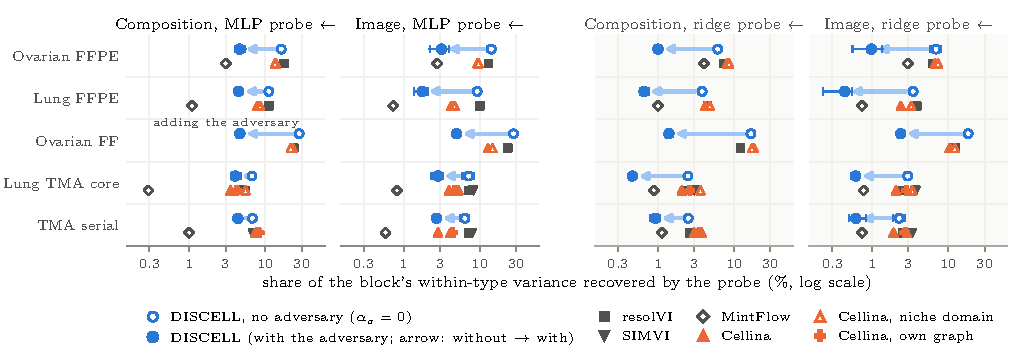
\includegraphics[width=\textwidth]{figures/fig_probe_data}
\caption{What the adversary removes from the intrinsic latent, per section. For each block and probe, the share of the block's within-type variance that the held-out probe explains from $\vz$ beyond the permutation floor ($1 - e^{-2\,\mathrm{excess}}$), in \% on a logarithmic scale: DISCELL without the adversary ($\alphaa = 0$, two seeds; open circle), with an arrow to DISCELL with it (the final fits, three seeds; filled circle), each with its range over seeds, and below them the comparison methods on the same section. The ridge probe (right, shaded) is the secondary read. Arrows point toward the better direction. On the serial section, the Cellina rows and MintFlow are the core's models transferred. SIMVI and MintFlow are absent on the sections where they could not be run (\cref{tab:baselines}). The values, and the fraction of the uncontrolled excess left, are in \cref{tab:probe}.}
\label{fig:probe-data}
\end{figure*}

\paragraph{The cell cycle.}
The cycle is an intrinsic state that the lineage labels do not encode, and it is carried by $\vz$ and not by $\vw$ (\cref{tab:headline,tab:headline-full}). The difference between the two holds at every leak fraction of the grid on every section, the serial section included (\cref{fig:breakdown-data}). A linear regression on the leading principal components of the counts explains less of the cycle scores than $\vz$ does on three sections, but more on the fresh-frozen section, the deepest ($83\%$ of their variance, against $74$ to $77\%$ for $\vz$). The cycle scores are not ground truth: they are gene-set scores of the cell's own segmented counts (\cref{app:readouts}), so transcripts leaked from cycling neighbours and expression induced by the environment raise them too, and the cycling set is chosen by them. That the response, close to its prior mean, a function of the neighbourhood (\cref{sec:results-w}), explains almost none of their within-type variance says that little of this axis follows the neighbourhood as the response represents it; it does not make the axis the cell's own, since $\vz$ is encoded from the same counts and would carry a leaked cycle signal, which the neighbours' types do not register. The sweep varies the leak fraction the model assumes, not the scores, so the asymmetry holding across it shows that the allocation does not depend on that assumption, not that the scores are free of leaked transcripts.

\paragraph{Merged subtypes.}
The lineage labels merge states and locations into their lineage, so the merged sublabels are held-out targets with a known allegiance: a state should be read from the intrinsic state, a location from the response (\cref{app:subtype}). On the primary section, where the sublabels are curated, the locations and two of the three tumour states follow it: the response, and equally its prior mean, separates tumour- from stroma-associated fibroblasts and endothelial cells (on two seeds of three by the pre-set call), and $\vz$ separates proliferating and inflammatory tumour cells (on every seed). The exceptions are states that also occupy a region, which both latents read: VEGFA$^+$ tumour cells on the primary section and three tumour-state clusters on the fresh-frozen section, while on the TMA core myofibroblasts among adventitial fibroblasts are read better from the response than from $\vz$. Merging such a state into its lineage moves part of it into the context regression, which is the cost of lineage labels anticipated in \cref{sec:setting,sec:invariance}.

\subsection{What the Response Carries}
\label{sec:results-w}
\readorder{7}
% manifest rows 6-8 (transport mean read, Read A, Read B), 14 (atlas, GO localisation), 15-17 (external criteria), 37 (held-out tiles)

\paragraph{Transport.}
\flag{TRIM}{about 450 words; Read A, twin margin and fold counts to app:response} \flag{REVIEWER}{keep the held-out-tiles read beside the headline read (decided 09-30)} The response is read through what the model predicts when a cell type is moved from one niche to another. For each type and pair of niches, the model's prediction holds the source cells' intrinsic state fixed and moves the prior mean of the response and the foreign influx to the target niche, and it is scored against the observed difference in the type's mean expression between the two niches, relative to the noise ceiling, the share of that difference that is reproducible between two random halves of the cells (\cref{app:readouts}). Over the panels whose ceiling is high enough to be read, the prediction recovers $0.65$ to $0.73$ of the ceiling (\cref{tab:headline}); its intervals (\cref{tab:headline-full}) have a coverage nearer $0.8$ than $0.95$ at the ceilings of real panels (\cref{app:readouts}). On the first seed, the response programmes alone recover $0.52$ to $0.64$ of the ceiling and the leakage alone $0.21$ to $0.39$ (\cref{tab:cellina-cf}); the two parts are not additive, but the programmes carry the larger share on every section. The full prediction's margin over the leakage alone holds across most of the sweep, but its margin over the programmes alone cannot be graded by it, so the sweep leaves open whether the leakage term adds to the prediction beyond the programmes (\cref{sec:results-sweep}). At the level of single cells, the decoded source cells, transported, close $0.70$ to $0.83$ of the gap, in maximum mean discrepancy, between the untransported cells and the target cells, each target cell decoded at its own posterior, where the target type's mean profile closes between $-1$ and $0.29$ (Read A, the median over panels); and for each target cell, the transported source cell nearest to it in $\vz$ is closer to the target's own decode than a random transported source cell, the median distance being $39$ to $46\%$ smaller (the twin margin). The transport reads are cross-fitted over spatial folds, but most of the scored cells lie in the model's training tiles. Scored on held-out tiles only, the fraction of the ceiling moves in both directions: in the trusted tier it lies above the published interval on $3$ of the $9$ fits with both reads, below it on $4$ and inside it on $2$, and over all panels above on $8$ of $11$, below on $2$ and inside on $1$; Read A is lower on held-out tiles on $11$ of $12$ fits, and the twin margin moves by at most $0.024$ (\cref{fig:transport-heldout}, \cref{tab:transport-heldout}). An in-sample advantage of the model would lower the held-out reads throughout; the fraction of the ceiling does not move that way, while Read A does. The held-out pool is also a quarter smaller, with fewer trusted panels. We keep the published read and report the other beside it.

\paragraph{Programmes.}
\flag{MOVE}{GO lean is descriptive and off-thread; one sentence here, rest in app:response} The response has two to five effective programmes per section, and the first is reproduced across seeds (\cref{tab:headline}, \cref{tab:breakdown-traj}). Its genes lean toward extracellular products and away from nuclear ones on the ovarian FFPE, lung and TMA sections, on every seed (rank-biserial effect $0.08$ to $0.22$ and $-0.12$ to $-0.19$), and toward plasma-membrane products on eight of those nine fits (\cref{app:response}). On the fresh-frozen section the extracellular lean fades from positive to null across the three seeds, so it is not a finding there. A lean toward secreted and membrane genes is also what a gene-specific leak would produce, which the sweep cannot separate (\cref{sec:generative}), so the lean is reported as a description, not as evidence of a response.

\paragraph{External criteria.}
\flag{MOVE}{criteria detail to app:response; keep the leakage-alone and not-specific caveats} Three criteria taken from other models' papers, two of them comparison methods here, are applied to our fits (\cref{app:response}). Ligand and receptor genes take a larger share of the between-niche shift than other genes in the leakage channel on every section and seed (rank-biserial effect $0.18$ to $0.28$), and also in the response channel on the ovarian FFPE, lung and TMA sections ($0.12$ to $0.18$); on the fresh-frozen section the response's lean is small ($0.01$ to $0.03$) and not significant in any seed by the per-seed rank test. The breakdown test is a different one, an interval for the mean over the three seeds of the difference in share, resampled over tiles; it excludes zero up to $\kappa = 0.1$ and not from $\kappa = 0.2$, where the lean breaks down (\cref{fig:breakdown-data}). The criterion that ligand--receptor genes respond more is thus reproduced by leakage alone on every section. The niche is read far more from the response than from the intrinsic state: by the same nearest-neighbour estimator as the guard of \cref{tab:headline}, on another sample of held-out cells and against its own within-type floors (\cref{app:response}), the response carries $0.41$ to $0.63$ nats of information about the niche and $\vz$ $0.06$ to $0.11$, on all four sections, the lung section included. On the primary section, the response's predicted shift of each gene follows the ordered bands of tumour density across the section more closely than it follows the in-plane coordinate least correlated with them (mean $|\tau|$ of $0.78$ to $0.81$ against $0.51$ to $0.56$), and the contrast holds across the leakage grid (\cref{fig:breakdown-data}). It holds in tumour cells and macrophages and fails in the merged fibroblast class, whose stromal half lies along the bands. The contrast is not specific to the response: predictions from the intrinsic state and from depth alone also follow the bands more than the false axis, with a lower true-axis $|\tau|$ ($0.57$ to $0.68$) but a difference of similar size.

\paragraph{The per-cell channel.}
\flag{KEEP-CORE}{thread point 4: per-cell channel closed by design, stated as a scoped result} At the operating point the response posterior stays at its prior: its own deviation adds one part in a thousand or less to held-out reconstruction (\cref{tab:recon-modes}), and its per-cell divergence, though spatially organised within a fit, ranks different cells in different seeds (\cref{app:kl-maps}). A simulated per-cell response, planted along the response programme in a tenth of one type's cells and unpredictable from the niche, is not detected by the rule fixed in advance at any strength up to twice the niche effect, and it is increasingly absorbed by the intrinsic state as it grows (\cref{app:planted-percell}, \cref{fig:planted-percell}). At $\alphaw = 0.1$ the per-cell channel is therefore closed by design, not by the data. On the ovarian FFPE, fresh-frozen and TMA sections the response and its prior mean also read the merged sublabels alike, within $0.07$ in AUC, with one exception on the TMA core (\cref{app:subtype}), so the response readouts above are readouts of the context regression $\mpsi(\vc_i, t_i)$ there (\cref{sec:objective}). On the lung section they are not only that: the response separates clusters within three lineages better than its prior mean does (AUC $0.67$ to $0.73$ against $0.55$ to $0.59$), although its own deviation adds as little to reconstruction as elsewhere. Lowering the weight opens the channel at a cost in agreement with type (\cref{app:sensitivity}).

\subsection{The Leakage Sweep}
\label{sec:results-sweep}
\readorder{5}
% manifest rows 9-10 (kappa sweep, kappa-survival), 11 and 21-23 (sensitivity), 18 (marker pairs), 38 (breakdown points)

Every section was refitted at each of the six leak fractions with three seeds. The claimed contrasts across the grid are drawn in \cref{fig:breakdown-data}; the diagnostics are drawn in \cref{fig:kappa-sweep} of the appendix, with their values in \cref{tab:kappa-sweep}. The diagnostics move smoothly along the grid: held-out reconstruction is nearly flat up to the operating point and falls beyond it, the mirror $R^2$ falls on every section, the cycle $R^2$ of $\vz$ stays within its seed range and that of $\vw$ near zero, and the response's information about the niche declines slowly. The response programmes survive the grid, their overlap with a reference fit at the operating point staying comparable to the overlap between seeds there (\cref{tab:breakdown-traj}). Magnitudes carry no breakdown point and are reported as trajectories (\cref{app:sweep}): the transport fraction of the ceiling is lower at $\kappa = 0$ than at the operating point, peaks between $\kappa = 0.05$ and $0.2$, and at $\kappa = 0.4$ is below its value at $\kappa = 0$ only on the primary section.

\begin{figure*}[t]
\centering
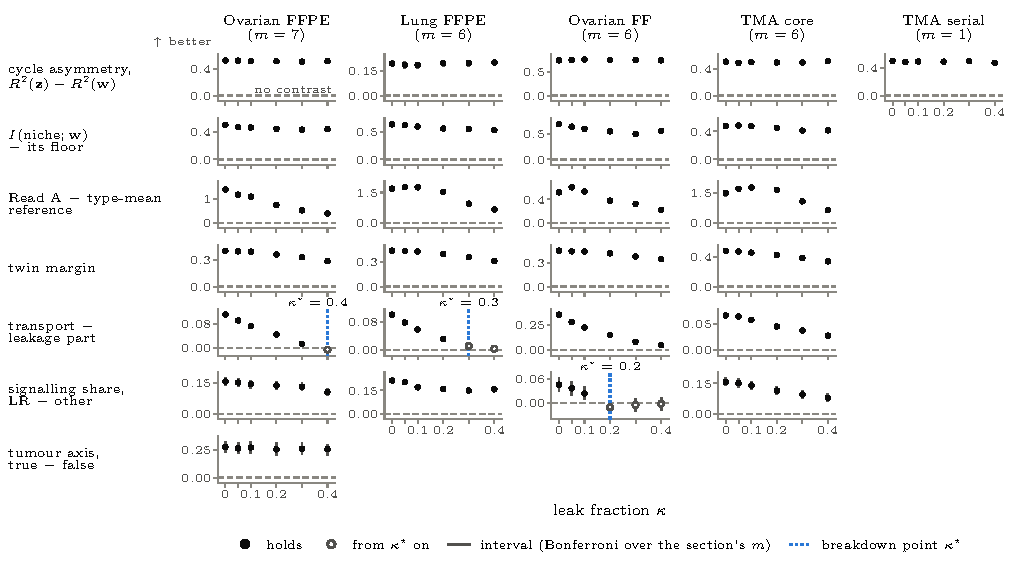
\includegraphics[width=\textwidth]{figures/fig_breakdown_data}
\caption{The claimed contrasts across the leakage sweep, the measured counterpart of \cref{fig:breakdown}. Rows: contrasts; columns: sections, with $m$ the number of contrasts in the section's set. At each $\kappa$, the mean over three seeds and its interval (spatial block bootstrap over tiles, two-sided, Bonferroni-adjusted over the section's $m$ contrasts); dashed, zero. Filled: the contrast holds at that grid point (every seed has its sign at $\kappa = 0$ and the interval excludes zero); hollow: from the breakdown point $\kappa^\star$ on (dotted). Each panel has its own vertical scale, which always includes zero, so an interval far from zero can be shorter than its marker. Arrows point toward the better direction: every contrast is signed so that it claims the side above zero. An empty panel: the contrast is not in that section's set. The transport prediction's margin over its programme part is not drawn: it is zero at $\kappa = 0$ by construction and is reported as a trajectory (\cref{tab:breakdown-traj}). The breakdown points are listed in \cref{tab:breakdown}.}
\label{fig:breakdown-data}
\end{figure*}

\paragraph{Breakdown points.}
Every claimed contrast holds at every leak fraction of the grid on every section, with two exceptions (\cref{fig:breakdown-data}, \cref{tab:breakdown}): the response's lean toward ligand--receptor genes on the fresh-frozen section, which breaks down at $\kappa = 0.2$, and the transported prediction's margin over its leakage part on the primary and lung sections, which breaks down in the upper half of the grid because a seed changes sign. The cycle asymmetry, the response's information about the niche, the two per-cell transport reads against their references and, on the primary section, the tumour-axis contrast are not explained away by leakage of the modelled form at any fraction up to $0.4$; leakage of another form is not ruled out (\cref{sec:sweep}). The transported prediction's margin over its programme part is a trajectory, not a claimed contrast: at $\kappa = 0$ no leakage is modelled, so the margin is zero by construction. Where a leak is modelled, the full prediction scores above its programme part in every seed on every section from $\kappa = 0.05$ to $0.2$; at the largest leak fractions it falls below it on the primary section and, in the mean, on the TMA core (\cref{tab:breakdown-traj}, \cref{app:sweep}).

\paragraph{Marker pairs.}
The marker-pair contrast is likewise a trajectory, of the decode (\cref{tab:breakdown-traj}). It compares the change in the rate at which mutually exclusive marker pairs are both detected in one cell, from the raw counts to the corrected decode, with the same change for control pairs that are expressed together (\cref{app:readouts}). It is negative at every grid value on the lung, fresh-frozen and TMA sections and positive on the ovarian FFPE section, and it is already present at $\kappa = 0$, where the decode removes no leakage; it therefore measures what decoding does to the counts, not what the leak correction removes, and is given no breakdown point. The correction's own effect at the operating point lowers exclusive and control double positives alike, although exclusive ones fall relative to control ones on every section, so the data do not show a removal specific to exclusive pairs (\cref{app:response}).

\paragraph{The form of the leak and other assumptions.}
Refitting the primary section with the leak's rate set per cell, from the neighbours' depth or density relative to the cell's own, or per gene at the same mean rate, moves no read by more than $1.3$ seed standard deviations of the final configuration (\cref{fig:sensitivity}; the values are in \cref{tab:sensitivity}). A fixed false-positive floor, a background rate per section, leaves the diagnostics in place but lowers the primary section's transport read from $0.65$ to $0.50$, a move of $8.3$ standard deviations and the largest of any arm, and less when the floor is scaled by cell area; on the TMA core it leaves transport in place. The transport read on the primary section is therefore sensitive to a background term the model does not have (\cref{app:sensitivity}).

\subsection{Comparison with Other Models}
\label{sec:results-baselines}
\readorder{4}
% manifest rows 4 and 34-36 (baseline battery, Cellina variants and counterfactual)

\Cref{fig:battery} scores every method by the same read-outs (the values are in \cref{tab:battery}), and \cref{fig:tradeoff} sets two of them against each other: how much within-type neighbour composition the intrinsic latent carries, by the probe of \cref{sec:invariance}, and how much within-type cell-cycle state it keeps. The comparison methods were fitted on our held-out cells as well (\cref{sec:setup}), so none of their reads is a held-out read. A DISCELL fit, its evaluations included, is up to $2.6$ times faster than the fastest competing model, Cellina, on three of the four sections, and slower than Cellina on the fresh-frozen section; it is over a hundred times faster than MintFlow wherever MintFlow could be run (\cref{tab:timing}).

\begin{figure*}[t]
\centering
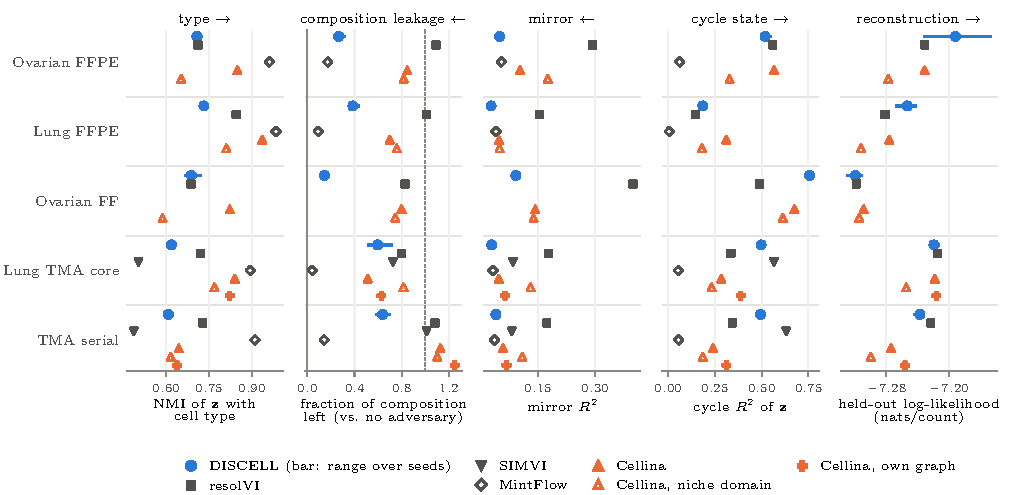
\includegraphics[width=\textwidth]{figures/fig_battery}
\caption{\flag{MOVE}{to app:baselines beside tab:battery; fig:tradeoff and fig:separation carry the thread} Every method on the same read-outs, at lineage labels, on the held-out cells of each section: NMI of the intrinsic latent with the type; the nonlinear probe's composition excess as a fraction of that of DISCELL without the adversary (solid at $0$, dashed at $1$); mirror $R^2$; cycle $R^2$ of the intrinsic latent on the top-decile cycling set; held-out reconstruction in nats per count. Markers as in \cref{fig:tradeoff}; DISCELL is the mean over three seeds with its range. Arrows point toward the better direction. The comparison methods are fitted on our held-out cells too, so their reads are not held-out reads. MintFlow's reconstruction is not reported, its stored value having been found invalid; refits are running (\cref{app:baselines}) \pending{MintFlow refits with the corrected export}, and SIMVI has no count decoder; methods are absent on the sections where they could not be run (\cref{tab:baselines}). The values are in \cref{tab:battery}.}
\label{fig:battery}
\end{figure*}

\begin{figure*}[t]
\centering
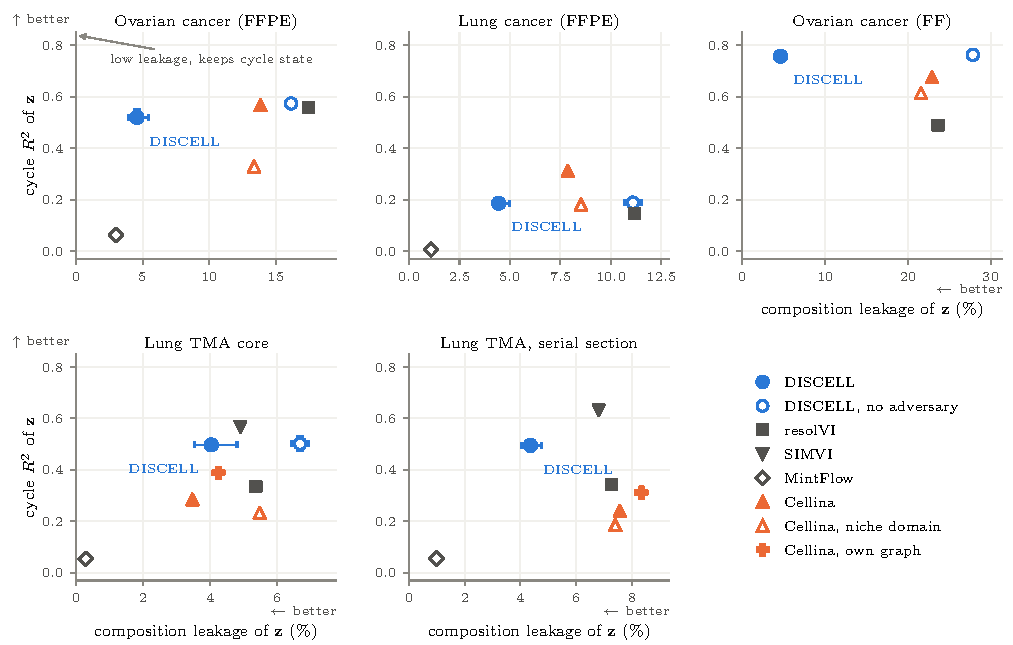
\includegraphics[width=\textwidth]{figures/fig_tradeoff}
\caption{\flag{KEEP-CORE}{thread point 4: less niche in z while keeping within-type state} Composition leakage of the intrinsic latent against the cell-cycle state it keeps, per section. \emph{Horizontal}: share of the within-type variance of neighbour composition that the held-out nonlinear probe explains from the intrinsic latent beyond the permutation floor ($1 - e^{-2\,\mathrm{excess}}$, in \%; \cref{tab:probe}). \emph{Vertical}: cycle $R^2$ of the intrinsic latent on the top-decile cycling set (\cref{tab:battery}). DISCELL: mean over three seeds, bars the range; open circle: DISCELL without the adversary (not read on the serial section). A method can be low on leakage by keeping little within-type state; DISCELL is low on leakage while keeping it. SIMVI and MintFlow are shown where their whole-section fits exist. Arrows point toward the better direction.}
\label{fig:tradeoff}
\end{figure*}

\begin{figure*}[t]
\centering
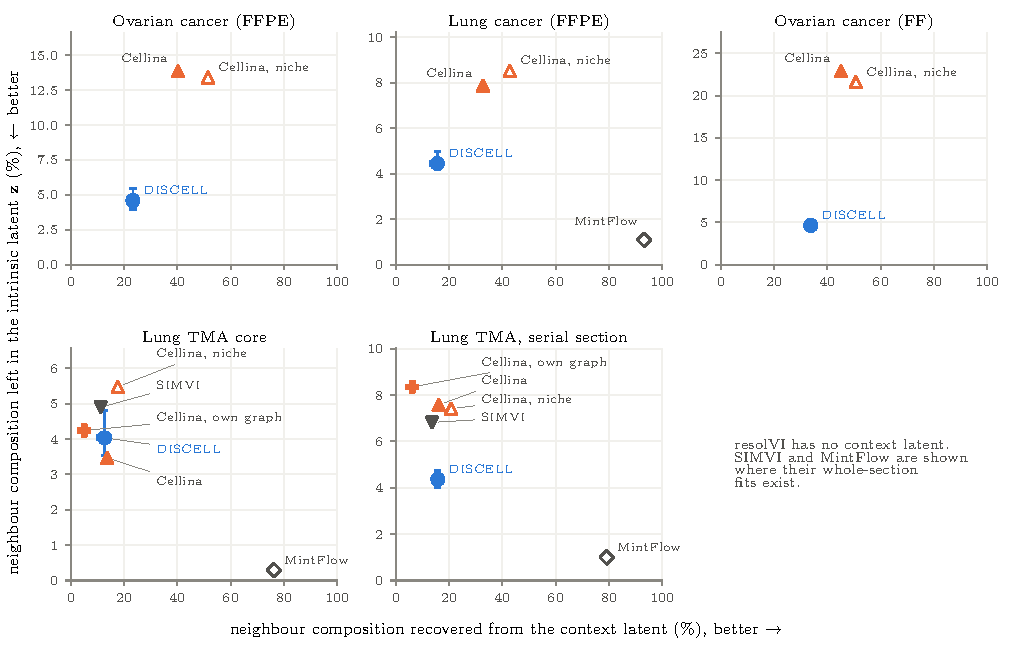
\includegraphics[width=\textwidth]{figures/fig_separation}
\caption{\flag{KEEP-CORE}{thread point 4: the context side graded like the intrinsic side} Neighbour composition in the context latent against the composition left in the intrinsic latent, per section. \emph{Horizontal}: share of the within-type variance of neighbour composition that the held-out nonlinear probe explains from each method's context latent beyond the permutation floor ($1 - e^{-2\,\mathrm{excess}}$, in \%; \cref{tab:context}). \emph{Vertical}: the same probe on the intrinsic latent, the horizontal axis of \cref{fig:tradeoff} (\cref{tab:probe}). A method that separates the two sits at the bottom right; arrows point toward the better direction. Markers as in \cref{fig:tradeoff}; DISCELL: mean over three seeds, bars the range. resolVI has no context latent; SIMVI and MintFlow are shown where their whole-section fits exist. MintFlow's intrinsic latent is close to a type label (\cref{tab:battery}).}
\label{fig:separation}
\end{figure*}

\paragraph{How to read the comparison.}
No single read-out ranks the methods; the pair in \cref{fig:tradeoff} does. On every section, each method that leaks less composition into its intrinsic latent than DISCELL keeps less cycle state (MintFlow, at a cycle $R^2$ of at most $0.06$; Cellina on the TMA core), and each that keeps more leaks more (Cellina on the FFPE sections, resolVI on the ovarian one, SIMVI on the TMA sections, narrowly on the core). DISCELL is never beaten on both, and is best on both on the fresh-frozen section; MintFlow is unbeaten too, but with almost no cycle state. DISCELL also has the lowest mirror $R^2$ on every section but the serial one (\cref{fig:battery}), though not the highest agreement with type.

\paragraph{Niche information in the intrinsic latent.}
\flag{REVIEWER}{keep the unfavourable rows: Cellina cycle, MintFlow residual, TMA core tie} On the ovarian FFPE, lung and fresh-frozen sections, DISCELL's intrinsic latent carries far less within-type neighbour composition than resolVI's or Cellina's, by both probes: the nonlinear probe recovers at most $5.5\%$ of its within-type variance, against $7.9$ to $24\%$ for the two comparison methods (\cref{tab:probe}). resolVI, with a single cell latent, serves as the reference of a model that does not separate the two. On the TMA core, where little leaks to begin with, the nonlinear residuals are close together and Cellina's is just below DISCELL's lowest seed, while the linear probe still finds several times less in DISCELL's latent than in resolVI's, Cellina's or SIMVI's; on the serial section only MintFlow's nonlinear residual is below DISCELL's. DISCELL keeps within-type state while doing so, although not the most of it everywhere (\cref{fig:tradeoff,tab:battery}): its cycle $R^2$ is the highest of all methods on the fresh-frozen section, while Cellina's is higher on the ovarian FFPE and lung sections, resolVI's on the ovarian FFPE section, and SIMVI's on the TMA core and its serial section, where SIMVI's latent also carries more composition. MintFlow reaches the lowest composition residuals of all, but its cycle $R^2$ is close to zero and its NMI with type high: its intrinsic latent is close to a type label. Cellina's NMI with type is higher than DISCELL's on every section, which its classifier on the intrinsic latent encourages, and its context latent mirrors its intrinsic latent more. Given our niche label as its domain, its best case on the probe, Cellina's adversary does not consistently lower its composition residual and lowers its NMI with type and its cycle $R^2$ on every section (\cref{app:baselines}).

\paragraph{Niche information in the context latent.}
Graded the other way, on each method's context latent (\cref{fig:separation,tab:context}), every context latent carries niche information beyond what the type carries. DISCELL's $\vmu_w$ holds less neighbour composition than Cellina's context latent on the ovarian FFPE, lung and fresh-frozen sections, about as much on the TMA core and its serial section, and far less than MintFlow's, which holds nearly all of it; it holds more of the image block than any comparison method's on the ovarian FFPE and lung sections, by both probes.

\paragraph{The counterfactual, head to head.}
Cellina also predicts expression under a rewired neighbourhood; scored by our transport reads on the same panels and draws, neither it nor DISCELL leads on every read (\cref{tab:cellina-cf}, \cref{app:cellina-cf}).
